\documentclass{beamer}
\usepackage[russian]{babel}
\usetheme{metropolis}

\usepackage{amsthm, amssymb}
\setbeamertemplate{theorems}[numbered]

\setbeamercolor{block title}{use=structure,fg=white,bg=gray!75!black}
\setbeamercolor{block body}{use=structure,fg=black,bg=gray!20!white}

\usepackage[T2A]{fontenc}
\usepackage[utf8]{inputenc}

\usepackage{hyphenat}
\usepackage{amsmath}
\usepackage{graphicx}

\AtBeginEnvironment{proof}{\renewcommand{\qedsymbol}{}}{}{}

\title{
Микроэкономика-I
}
\author{
Павел Андреянов, PhD
}

\begin{document}

\maketitle

\section{Программа курса}

\begin{frame}{Программа модуля}
\begin{itemize}
\item Теория Потребителя
\begin{itemize}
\item Модель: товары $x, y$ $\to$ полезность $U(x,y)$
\item Максимизация полезности
\item Предпочтения, спрос, эластичность...
\item CV, EV
\end{itemize}
\item Теория Производителя
\begin{itemize}
\item Модель: ресурсы $x, y$ $\to$ производство $F(x,y)$
\item Максимизация прибыли (минимизация издержек)
\item Технологии, предложение, эластичность...
\end{itemize}
\item Частичное равновесие
\begin{itemize}
\item налоги, потолки, DWL
\end{itemize}
\end{itemize}
\end{frame}

\begin{frame}{Люди и материалы}

Лектор: Павел Андреянов (pandreyanov@gmail.com/hse.ru)

Семинаристы: Даша

Учебники:
\begin{itemize}
\item Вэриан (V) и Ехил Рени (JR), есть русские версии
\item Бусыгин, Желободько, Цыплаков (BZC) том I,II
\item Мас Колел (MC)
\end{itemize}

Задачник -- Левина, Покатович

\end{frame}

\begin{frame}{Люди и материалы}

Прочие ресурсы:
\begin{itemize}
\item телеграм: \url{channel_micro_2023}, \url{forum_micro_2023}
\item офис аурз: TBD
\item консультации и тестовые контрольные
\item \url{pandreyanov.github.io/pashas_micro_one_lectures}
\end{itemize}

\end{frame}

\begin{frame}{Люди и материалы}

\begin{figure}[hbt]
\centering

\includegraphics[width=.6 \textwidth]{qrcode}
\end{figure}

\end{frame}

\section{Предисловие}

\begin{frame}{Предисловие}

Экономика это не физика, и не ветвь прикладной математики, а школа философской мысли, в которой некоторые рассуждения могут делаться при помощи математики. 

Но на сегодняшний день традиция такова, что мы думаем об экономике именно в терминах жестких математических моделей. 

\end{frame}

\begin{frame}{Предисловие}

Модели пишутся на языке мат. анализа, что позволяет этим моделям пересекать временные, языковые и культурные границы. 

Но само по себе использование мат. анализа не делает эти модели <<правильными>>  и, в конечном счете, оценка качества модели субъективна.

В экономике вообще нет <<правильных>> моделей. 

\end{frame}
%
%\begin{frame}{Предисловие}
%
%За последние полвека в экономике было создано большое количество конкурирующих моделей, некоторые из них открыто противоречащих друг другу. Эти модели постоянно обновляются, сменяют друг друга. 
%
%Это не признак незрелости экономической науки а, наоборот, ее достижение. 
%
%\end{frame}
%
%\begin{frame}{Предисловие}
%
%В физике такое случалось всего несколько раз и это чуть не привело к кризису  научной мысли. Например, Эйнштейн отказывался верить в то, что нет   <<правильной>> модели, объясняющей все наблюдаемые квантовые парадоксы. 
%
%Он утверждал, что через какое-то время нужная модель найдется, надо только подождать.
%
%\end{frame}
%
\begin{frame}{Предисловие}

Существует большое количество разнообразных моделей и у каждой есть свои достоинства и ограничения.

В этом курсе мы научим вас быть последовательными в рамках отдельно взятых моделей, а также немного разбираться в их многообразии.

\end{frame}

\section{План}

\begin{frame}{План на первую половину лекции}

\textbf{Модели поведения потребителя.}

Мы поговорим подробно о первых двух моделях (полезность и предпочтения) и, вскользь о третьей модели (выбор). Большой упор будет сделан на понятия непрерывности и выпуклости. (\alert{скорее всего тут время закончится})

Затем, мы попробуем отождествить некоторые из этих моделей между собой. В частности, будет обсуждена относительно простая прямая связь между полезностью и предпочтениями.

Вершиной этого блока будет обратная связь между предпочтениями и полезностью, так называемая, \alert{Теорема Дебре}. После нее надо сделать перерыв.

\end{frame}

\section{Что такое модель?}

\begin{frame}{Что такое модель?}

Модель - это упрощенная версия реальности, из которой специально убраны детали, иногда очень важные, для того чтобы изолировать и анализировать какой то один аспект этой (сложной) реальности. 

Сила модели идет не от ее детализации и сложности, а, наоборот, от ее простоты. Хорошая модель - это (максимально) простая модель, объясняющая феномен. 

Этот методологический принцип называется бритвой Оккама, хотя он был известен со времен Аристотеля.

\end{frame}

\begin{frame}{Что такое модель?}

К примеру, мы желаем изучить рынок жилья для студентов. 

Есть жилье поближе и подальше. Чем ближе тем лучше для студента, но также дороже. Также есть общественный транспорт, метро, велосипед...

Как студент принимает решение о выборе жилья?

\end{frame}

\begin{frame}{Что такое модель?}

Другой пример, я прихожу в супермаркет. 

Я могу купить мясо, рыбу, несколько овощей и фруктов. У меня есть определенный бюджет, но я могу из него выйти за счет кредитки.

Как я принимаю решение что купить и в каком количестве?

\end{frame}

\begin{frame}{Что такое модель?}

В этом курсе мы чаще всего будем делать предположение о \alert{конкурентном рынке} - это когда товары и ресурсы покупаются по стабильным (и \alert{экзогенным}, от греч. -genēs рожденный и  exō- снаружи) рыночным ценам. 

В более общем смысле, агент не может повлиять своими действиями на состояние рынка, потому что он слишком мал по отношению к рынку.

Это конечно же неверно, но мы будем его предполагать, если не сказано иначе.

\end{frame}

\section{Три модели потребителя}

\begin{frame}{Три модели потребителя}

Три конкурирующих модели поведения потребителя:

\begin{itemize}
\item полезность (классика)
\item предпочтения (нео)
\item выбор
\end{itemize}

Различия между ними скорее философские, но мы все равно преподаем их как часть традиционного курса микроэкономики.

\end{frame}

\section{Полезность}

\begin{frame}{Полезность}

В модели полезности (классика) у каждого агента в голове зашита функция полезности, которая переводит любой \alert{портфель} или \alert{корзину}  потребительских товаров (или совсем абстрактно \alert{альтернатива}) в вещественное число с мистической единицей измерения \alert{утили}.

\end{frame}

\begin{figure}[hbt]
\centering
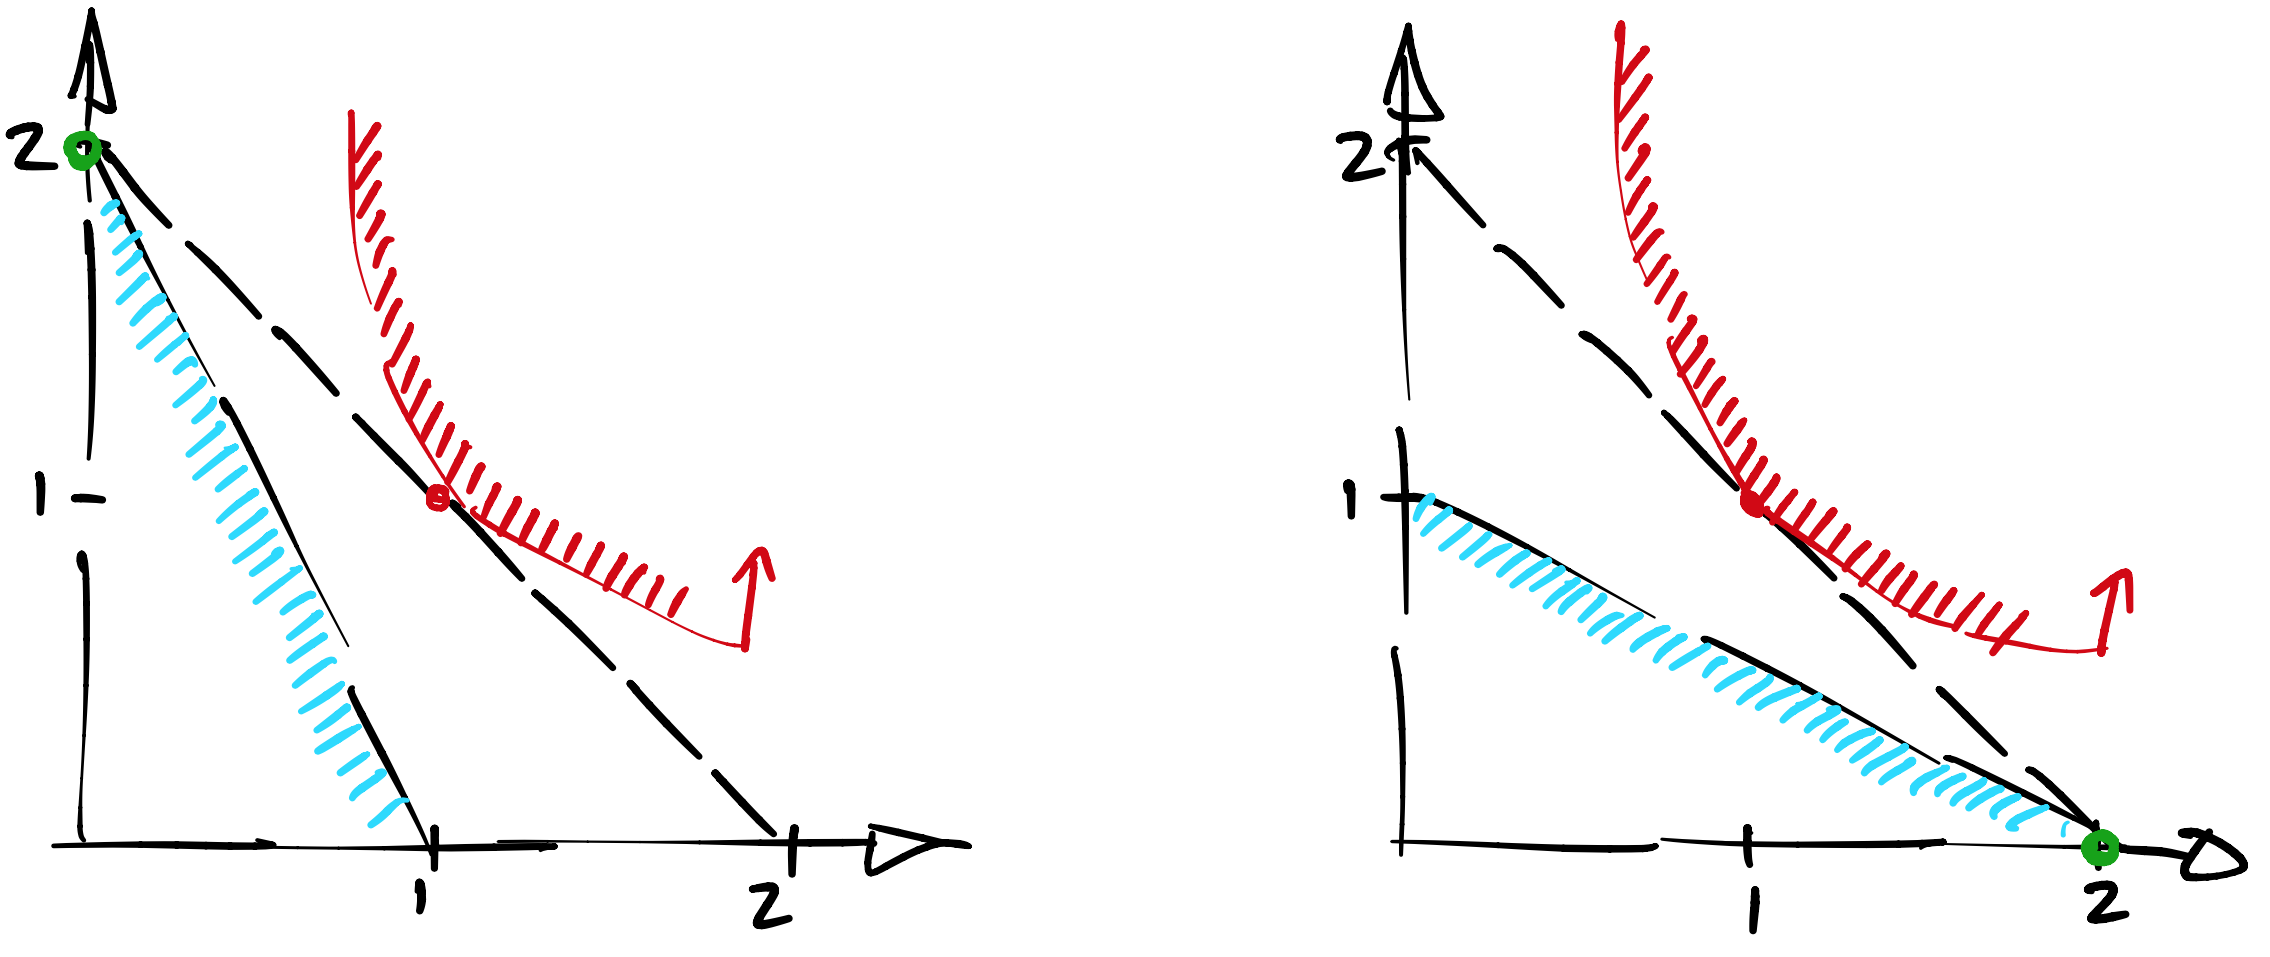
\includegraphics[width=1 \textwidth]{pic2}
\end{figure}

\begin{frame}{Полезность}

Например, у меня на выбор есть

\begin{itemize}
\item 3 куба, 1 круг = 8 утилей
\item 12 конусов = 60 утилей
\item 1 конус, 4 круга = 3 утиля
\end{itemize}

Агенты сравнивают утили и принимают экономические решения, дабы их максимизировать. В данном случае мы выберем 2ой вариант на 60 утилей.

Это самая старая модель, поэтому мы будем называть ее \alert{классической}.

\end{frame}

\begin{frame}{Полезность}

Полезность определена с точностью до монотонного преобразования. Это серьезная проблема, это значит, что модель невозможно толком \alert{откалибровать} или \alert{оценить}.

\end{frame}

\begin{frame}{Полезность}

Действительно, все нижеперечисленные полезности неразличимы с точки зрения наблюдателя. 
\begin{itemize}
\item $x^2 y^3$
\item $2 \log x + 3 \log y$
\item $2 \log x + 3 \log y + 1$
\item $5(2 \log x + 3 \log y) + 1$
\end{itemize}

Если модель нельзя оценить по данным, это однозначно <<плохая>> модель. Экономисты всегда-всегда пытаются от этого избавиться.

\end{frame}

\begin{frame}{Полезность}

Как правило, в классической модели все координаты $x,y$ неотрицательные, потому что непонятно, что значит потребить $-1$ яблок. Это иногда пишется явно, а иногда умалчивается для экономии чернил. 

Всегда подразумеваем что $x,y \geqslant 0$, если не сказано обратное. Но только для потребителя, потому что производитель может потребить -10 яблок, чтобы произвести яблочный сок.

\end{frame}

\begin{frame}{Полезность}

Полезность можно также задать табличкой

\begin{center}
\begin{tabular}{ |c c c| } 
 \hline
 1 яблоко&+ \ 1 груша & = 3 утиля \\ 
 2 яблока&+ \ 1 груша & = 4 утиля \\ 
 1 яблоко&+ \ 2 груши & = 5 утилей \\ 
 \hline
\end{tabular}
\end{center}

Потренируемся в монотонном преобразовании утилей?

\end{frame}


\section{Предпочтения}

\begin{frame}{Предпочтения}

В модели предпочтений от агентов требуется, казалось бы, меньше. Они должны в моменте сравнить два портфеля и назвать лучший. Другими словами, они должны озвучить предпочтения.

Мы будем называть эту модель \alert{неоклассической}.

\end{frame}

\begin{frame}{Предпочтения}

\begin{figure}[hbt]
\centering
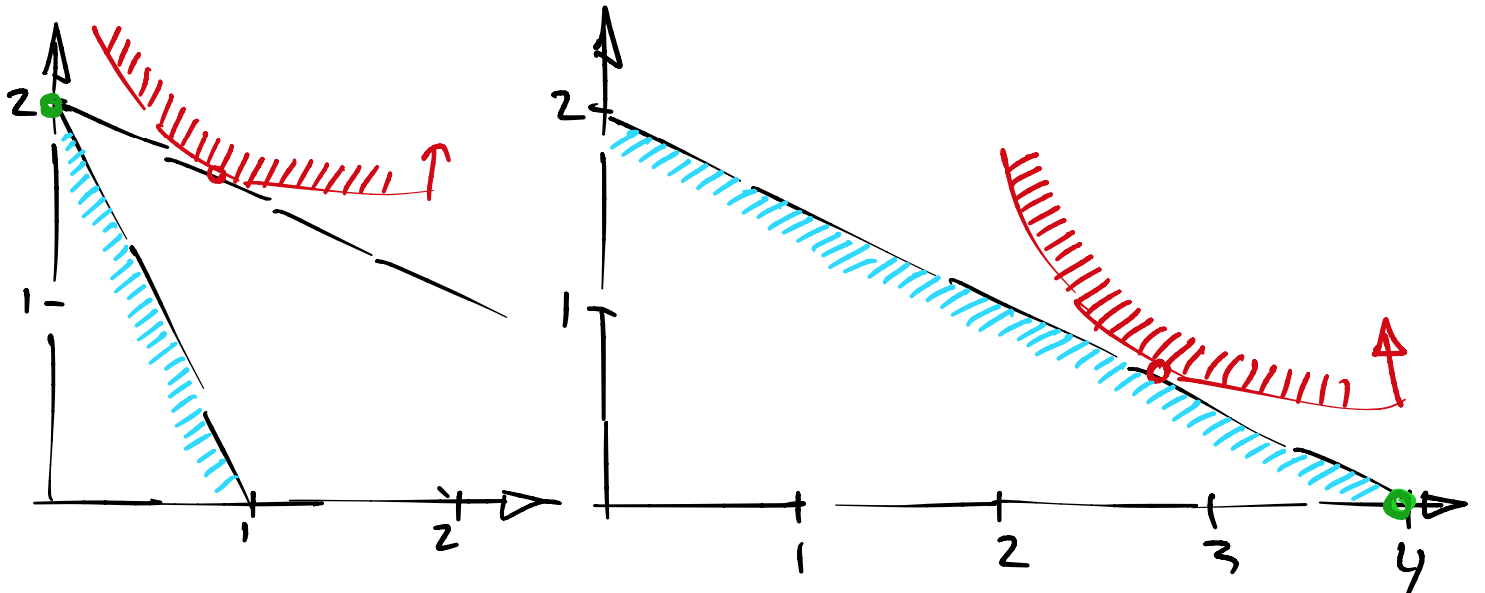
\includegraphics[width=.7 \textwidth]{pic4}
\end{figure}

\end{frame}

\begin{frame}{Предпочтения}

Этот минимализм обманчив. Чтобы оставаться экономическими агентами, они должны помнить все свои выборы, и не менять их на протяжении эксперимента.

Это матрица $n \times n$, где $n$ - это число возможных портфелей. Это очень много надо агенту запомнить.

Зато, здесь отсутствует проблема представления поведения потребителя двумя разными моделями, поэтому экономисты эту модель тоже очень любят.

\end{frame}

\begin{frame}{Предпочтения}

Для простоты пусть есть всего три альтернативы $a,b,c$, тогда я могу зафиксировать выбор таким образом:
$$\begin{array}{c|ccc}
 \succcurlyeq & a & b & c\\
 \hline
 a & 1 & 0 & 1\\
 b & 1 & 1 & 0\\
 c & 1 & 0 & 1
\end{array}$$

Значок $\succcurlyeq$ означает предпочтение. 

Запомним эту таблицу

\end{frame}

\begin{frame}{Предпочтения}

Для данной таблицы $$\succcurlyeq(a,b) = 0, \quad \succcurlyeq(b,a) = 1$$ что означает <<строгое>> предпочтение $b$ над $a$. 

Я буду использовать вот такой значок $b \succ a$ для <<строгого>> и вот такой значок $b \succcurlyeq a$ для <<нестрогого>> предпочтения, что означает
$$\succcurlyeq(a,b) = 0 \text{ или } 1, \quad \succcurlyeq(b,a) = 1$$

... вообще я могу писать просто скобки, без $\succcurlyeq$.

\end{frame}

\begin{frame}{Предпочтения}

Получается довольно элегантный язык предпочтений. 

Ставим в табличку $(x,y) = 1$ если агент проявил нестрогое предпочтение $x$ над $y$, например, добровольно поменял в эксперименте $y$ на $x$.

\begin{itemize}
	\item $(a,b) = 1$ и $(b,a) = 0$ это $a \succ b$
	\item $(a,b) = 0$ и $(b,a) = 1$ это $b \succ a$
	\item $(a,b) = 1$ и $(b,a) = 1$ это $b \sim a$
\end{itemize}

Ставим в табличку $(x,y) = 0$ если (тут нужно проявить фантазию) агент отказался менять $y$ на $x$ плюс <<эпсилон>>.

\end{frame}

\begin{frame}{Предпочтения}

Потренируемся у доски переводить полезности в предпочтения...

Пусть множество альтернатив это числа -2, -1, 0, 1; Заполните матрицу предпочтений для следующих функций полезности, как если бы вы проводили эксперимент над человеком с истинной классической полезностью над целыми числами

\begin{itemize}
\item полезность $x$
\item полезность $x^2$
\item полезность $|x|$
\item полезность $x^3$	
\end{itemize}

\end{frame}

\section{Выбор}

\begin{frame}{Выбор}

В модели выбора от агентов требуется принимать решения, максимально приближенные к реальности. Вам предлагают меню (\alert{menu}) из: $(a,b,c)$, $(a,b)$, $(a,c)$, $(b,c)$, $(a)$, $(b)$, $(c)$.

И вы просто вычеркиваете то, что вам точно не нравится. Все что вы не вычеркнули - это и есть ваш выбор (\alert{choice}). 

Эта модель требует от экономического агента знать не свою функцию полезности, и даже не $n^2$ готовых ответов, как в предпочтениях, а целых $2^n$ готовых ответов.

\end{frame}

\begin{frame}{Выбор}

\begin{figure}[hbt]
\centering
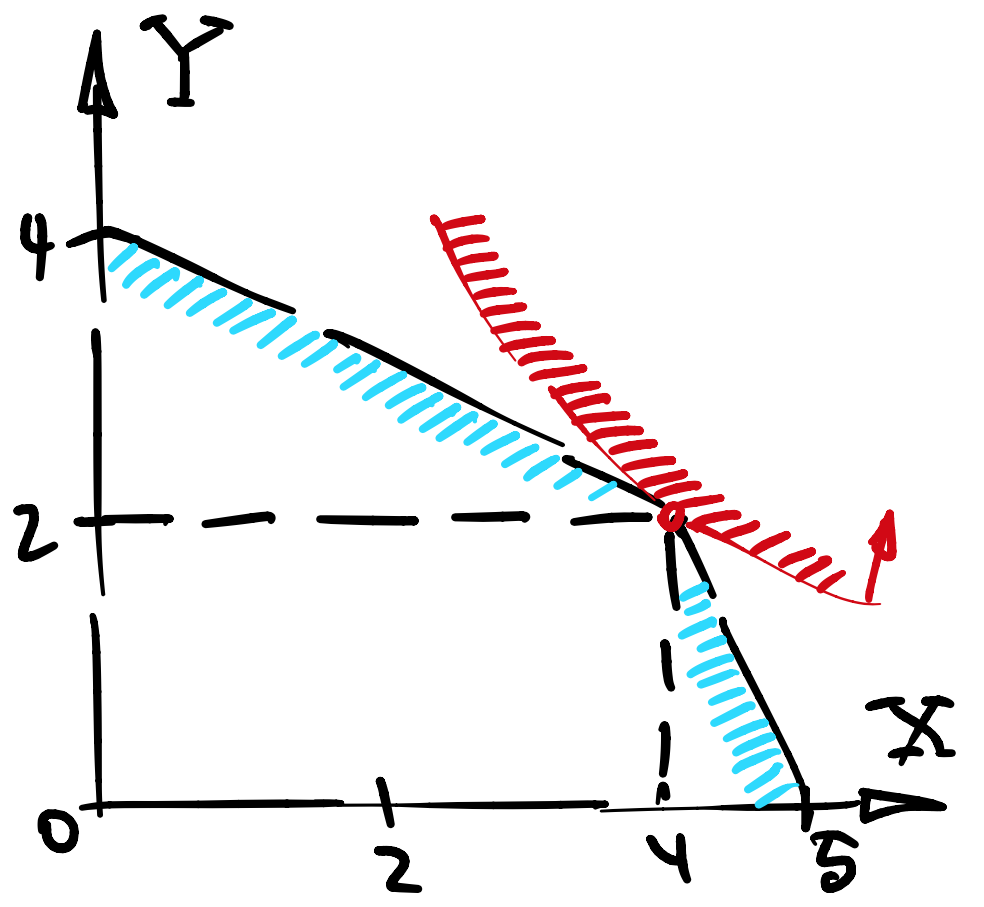
\includegraphics[width=.7 \textwidth]{pic3}
\end{figure}

\end{frame}

\begin{frame}{Выбор}

Потренируемся у доски переводить полезности в выбор...

Пусть множество альтернатив это наборы чисел (-2,1,2), (-1,1), (0,1), (1); Запишите выбор, как если бы вы проводили эксперимент над человеком с истинной классической полезностью над последовательностями чисел

\begin{itemize}
\item полезность $\sum_i x_i$
\item полезность $\sum_i x_i^2$
\item полезность $|x_0|$
\end{itemize}

\end{frame}

\begin{frame}{Выбор}

На самом деле, есть строгие определения того как спускать полезность в предпочтения и предпочтения в выбор (именно такая иерархия) однако я хотел чтобы вы сами догадались, вместо того чтобы запоминать их.

Они очень естественные и интуитивные.
\end{frame}

\section{Какая из моделей лучшая?}

\begin{frame}{Какая из моделей лучшая?}

Можно долго спорить, какая из этих моделей более или менее реалистичная. Правильный ответ - они все нереалистичные. 

\begin{itemize}
  \item агент должен знать ответы на все вопросы
  \item ответ не может меняться во времени
\end{itemize}

Реализм вообще не является добродетелью модели. Вся суть модели в том, чтобы подняться на другой уровень абстракции.
\end{frame}

\section{Потренируемся в моделировании}

\begin{frame}{Потренируемся в моделировании}
	Какую модель вы бы выбрали для описания следующих жизненных задач? и почему

\begin{itemize}
  \item купить продуктов в магазине
  \item выбора университета
  \item голосования в думу
  \item одежду отдать в приют или оставить себе
\end{itemize}	
	
\end{frame}

\begin{frame}{Потренируемся в моделировании}

Предположим, что вы выбрали утилитарную (классическую) модель.

Далее, вам нужно ответить на следующие вопросы

\begin{itemize}
  \item сколько вообще товаром
  \item какие доступны альтернативы
  \item что мы знаем про полезность/предпочтения/выбор
\end{itemize}	
	
\end{frame}

\section{Классическая модель}

\begin{frame}{Классическая модель}

Модель полезности обладает высоким уровнем абстракции

\begin{itemize}
\item начнем с одного агента
\item товары разделены на $n$ категорий
\item портфель/корзина/алътернатива это точка в $\mathbb{R}_{+}^{n}$	
\item категории, а также координаты обозначаются $x, y, z...$
\item соответствующие цены обозначаются $p, q, y...$
\item полезность обозначается $U(x,y,z, \ldots)$
\item множество доступных альтернатив $X \subset \mathbb{R}_{+}^{n}$
\end{itemize}


Плюсик в $\mathbb{R}_{+}^{n}$ означает неотрицательные значения потребления, мы иногда называем это множество \alert{первый/положительный ортант Евклидового пространства}.

\end{frame}

\begin{frame}{Полезность}

Таким образом, мы может сформулировать модель потребителя как абстрактную оптимизационную задачу, скажем, для трех товаров:
$$ U(x,y,z, \ldots) \to \max_{(x,y,z, \ldots) \in X}$$
Формально \alert{классическая  (утилитарная) модель} это пара: множество альтернатив $X \subset \mathbb{R}^n_{+}$ и полезность $U: X \to \mathbb{R}$.

Никаких дополнительных аксиом не требуется.

Множество альтернатив будет, как правило, зависеть от цен $p,q,r...$ и бюджета $W$ (от слова \alert{wage}).
$$ X = \{x,y,z... \in \mathbb{R}_{+}^{n}: p x + q y + r z + \ldots \leqslant W \}$$

\end{frame}

\begin{frame}{Пример 1}

У Пети есть 100 рублей. Он может купить яблоки ($x$) по цене 20 рублей за штуку либо груши ($y$) по цене 50 рублей за штуку. Петя получает полезность 2 за каждое яблоко и 3 за каждую грушу, но не получает никакой полезности за оставшиеся деньги. 

Попробуем записать это формально:

\begin{itemize}
  \item $X = \{(x, y) \in  \mathbb{N}^2_{+}: 20 x + 50 y \leqslant 100 \}$
  \item $U(x, y) = 2x + 3y$
\end{itemize}

Здесь $\mathbb{N}^2_{+}$ это \alert{решетка из целых значений}, потому что нельзя покупать нецелые яблоки и груши.

\end{frame}

\begin{frame}{Пример 2}

У Кати есть 24 часа в сутки, из которых она должна как минимум 8 часов поспать ($x$), a дальше она учится и занимается. Однако, на каждый час учебы ($y$) нужен один час отдыха ($z$), и наоборот, иначе время проходит зря.

Попробуем записать это формально:

\begin{itemize}
  \item $X = \{(x, y, z) \in  \mathbb{R}^3_{+}: x + y + z \leqslant 24 \}$
  \item $U(x, y, z) = \mathbb{I}(x \geqslant 8)\cdot \min(y,z)$
\end{itemize}

Здесь $\mathbb{I}(x \geqslant 8)$ это \alert{индикатор-функция}, принимающее значение 1 когда выражение в скобках выполнено, иначе 0.

\end{frame}

\section{Свойства полезности в $\mathbb{R}^n$}

\begin{frame}{Непрерывность}

Мы начнем с двух эквивалентных определений непрерывности.

\begin{definition}
Полезность $U$ \alert{непрерывна} в $X$, если для любого $x \in X$ множества $L_{+}(x)$ и $L_{-}(x)$ замкнуты, где
\begin{gather*} L_{+}(x) = \{y \in X: U(y) \geqslant U(x)\}\\
 L_{-}(x) = \{y \in X: U(y) \leqslant U(x)\}\end{gather*}
\end{definition}

Описанные выше множества $L_{+}(x)$ (или $L_{-}(x)$) - это подмножества допустимых альтернатив, которые не хуже (или не лучше), чем сам $x \in X$. 

Их часто называют \alert{Лебеговыми множествами} относительно точки $x$, $L_{+}(x)$ - верхним а $L_{-}(x)$ - нижним.

\end{frame}

\begin{frame}{Непрерывность}

\begin{figure}[hbt]
\centering
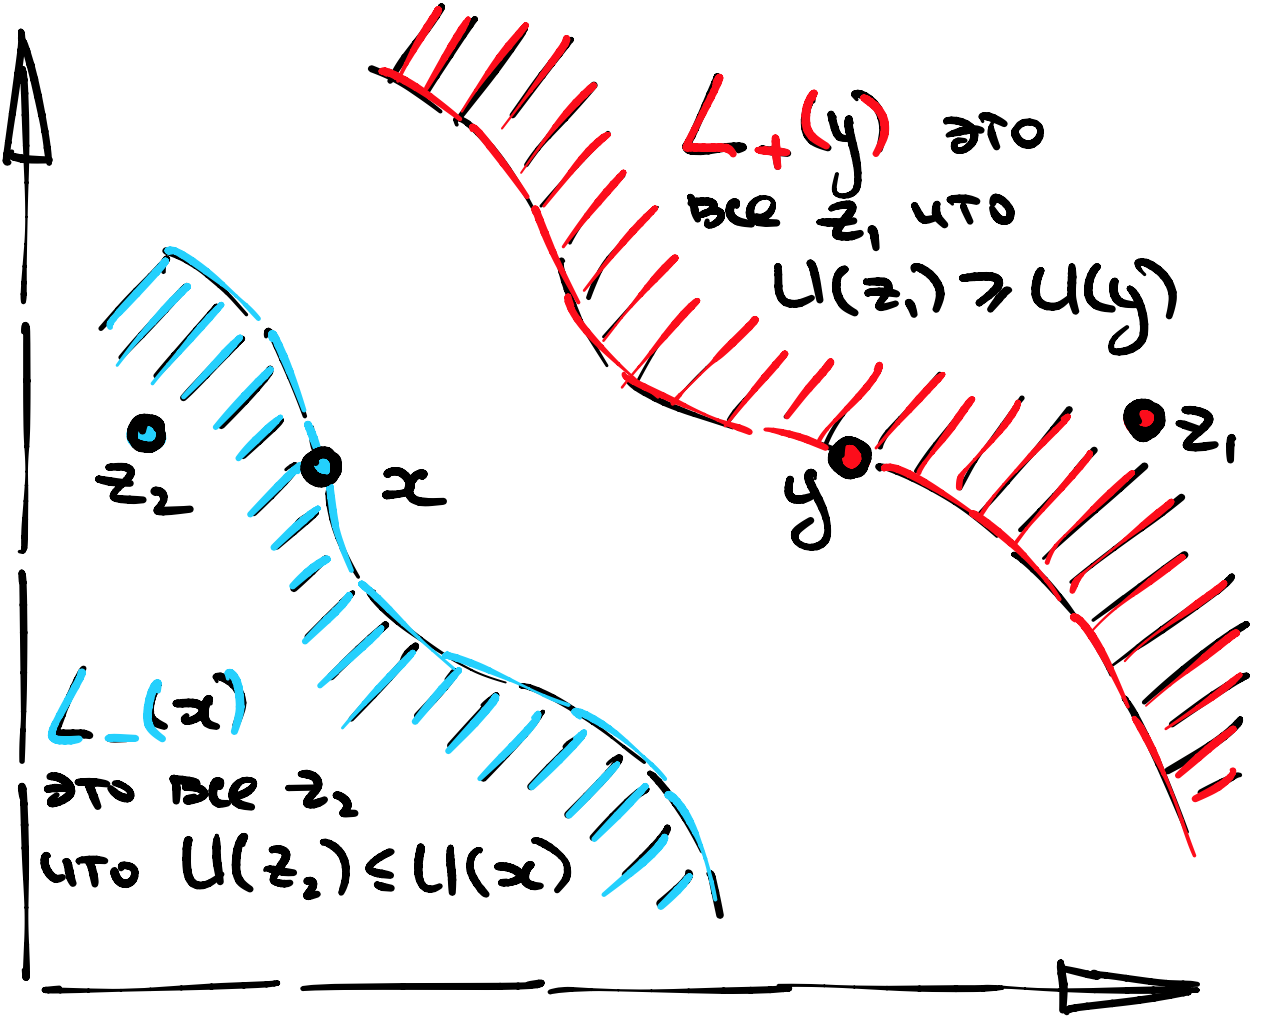
\includegraphics[width=.8 \textwidth]{lebeg_sets.png}
\end{figure}

\end{frame}

\begin{frame}{Непрерывность}

Эквивалентное (но только в Евклидовых пространствах) определение непрерывности можно дать на более знакомом вам с курса мат. анализа языке эпсилон-дельта.

\begin{definition} Полезность $U$ \alert{непрерывна} в $X$, если для любого $\varepsilon > 0$ существует $\delta >0$ такой что для любых $x, y \in X$: $$ ||x - y|| < \delta \quad \Rightarrow \quad ||U(x) - U(y)|| < \varepsilon.$$	
\end{definition}

Но оно практически бесполезно.

\end{frame}

\begin{frame}{Вогнутость}

Следующее важное определение - это вогнутость.

\begin{definition}
Полезность $U$ \alert{вогнута}, если для любых $x, y \in X$: 
$$ \forall \alpha \in (0,1): U(\alpha x + (1-\alpha) y)) \geqslant \alpha U(x) + (1-\alpha) U(y)$$
\end{definition}

Многие полезности уже вогнуты сами по себе, например: $ax + by, \min(x,y), \sqrt{xy}, x + \log y$, но некоторые такими не являются, например $\max(x,y)$, $x^2y^2$.

\end{frame}

\begin{frame}{Вогнутость}

\begin{columns}
\begin{column}{0.5\textwidth}
   Пусть пространство товаров $\mathbb{R}^{2}_+$, для простоты. Тогда график функции это такая поверхность. Можно сказать, что \alert{вогнутая функция это когда подграфик выпуклый}, либо, \alert{график вогнутой функции выглядит как колпак}. Еще одно правило - это \alert{график вогнутой функции находится под касательной плоскостью.}\end{column}
\begin{column}{0.5\textwidth}  %%<--- here
    \begin{center}
    рисунок в $\mathbb{R}^{n+1}$
     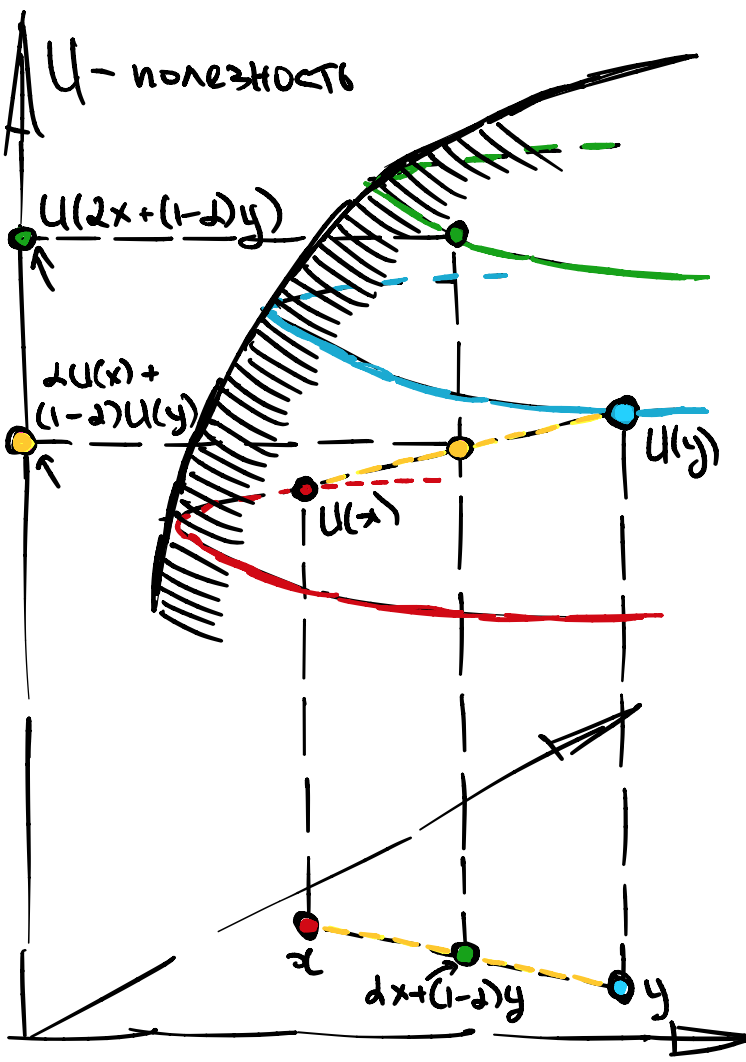
\includegraphics[width=.9\textwidth]{concave.png}
     \end{center}
\end{column}
\end{columns}

\end{frame}

\begin{frame}{Вогнутость}

В этом курсе я буду чаще всего пользоваться 2-мерным (1-мерным) пространством товаров, но когда мне надо будет посмотреть на функцию от этих товаров, будет получаться график в соответственно 3-мерном (2-мерном) пространстве.

\end{frame}


\begin{frame}{Вогнутость}

Постарайтесь не путать ситуацию когда вы смотрите только на область определения функции ($\mathbb{R}^{n}$) где живут верхние и нижние Лебеговы множества, с ситуацией когда вы смотрите на область определения с приклеенной к ней осью значений ($\mathbb{R}^{n+1}$) где живут график и подграфик функции.

\end{frame}

\begin{frame}{Вогнутость}

К сожалению, не все могут быстро в уме нарисовать график функции от двух переменных, а тем более от трех переменных, и сказать выглядит он как колпак или нет.

В таких случаях мы применяем \alert{критерий Сильвестра} (какого покажу на следующем слайде) для установления выпуклости/вогнутости дважды дифференциируемой функции.

\end{frame}

\begin{frame}{Вогнутость}

Если же функция вовсе не дифференциируема, как, например, $\min(x,y)$, нужно проявить смекалку: \alert {минимум вогнутых функций вогнут}, поскольку подграфик минимума это пересечение соответствующих подграфиков, а \alert{пересечение двух выпуклых множеств выпукло}. В данном случае первая вогнутая функция это $f(x,y) = x$, а вторая это $g(x,y) = y$. 

Вообще, \alert{линейные функции всегда вогнутые}, запомните.

\end{frame}

\begin{frame}{Критерий Сильвестра}

\begin{columns}
\begin{column}{0.5\textwidth}
   \alert{Джеймс Джозеф Сильвестер} (James Joseph Sylvester) английский и американский математик второй половины 19 века, профессор Университета Джон Хопкинс и позже Оксфорда. Изобрел матрицы, дискриминанты, и, собственно, критерий имени самого себя. \\ Этот критерий заключается в проверке отрицательной определенности матрицы Гесса.
\end{column}
\begin{column}{0.5\textwidth}  %%<--- here
    \begin{center}
     \includegraphics[width=1\textwidth]{sylvester.jpeg}
     \end{center}
\end{column}
\end{columns}

\end{frame}

\begin{frame}{Вогнутость}

Однако, с вогнутостью есть проблема. Три полезности

\begin{itemize}
  \item $x^2y^2$
  \item $\sqrt{xy}$
  \item $\log x + \log y$
\end{itemize}

задают одни и те же предпочтения однако 2 из них вогнутые а одна - вовсе нет.

Попробуйте определить какие?

Поэтому экономисты придумали свою собственную почти-вогнутость, или \alert{квази-вогнутость} (quasi- от лат. почти). Она, в отличие от истинной вогнутости, полностью оторвана от свойств графика функции.

\end{frame}

\begin{frame}{Квази вогнутость}

\begin{definition}
Полезность $U$ \alert{квазивогнута} в $X$, если $\forall x \in X$ верхнее Лебегово множество $L_{+}(x)$ выпукло. 
\end{definition}

И совершенно эквивалентное ему

\begin{definition}
Полезность $U$ \alert{квазивогнута} в $X$, если для любых $x, y \in X$ их линейная комбинация не хуже, чем худшая из двух:
$$ \forall \alpha \in (0,1): U(\alpha x + (1-\alpha) y)) \geqslant \min(U(x), U(y))$$

\end{definition}

\end{frame}

\begin{frame}{Квазивогнутость}
рисунок в $\mathbb{R}^n$
\begin{figure}[hbt]
\centering
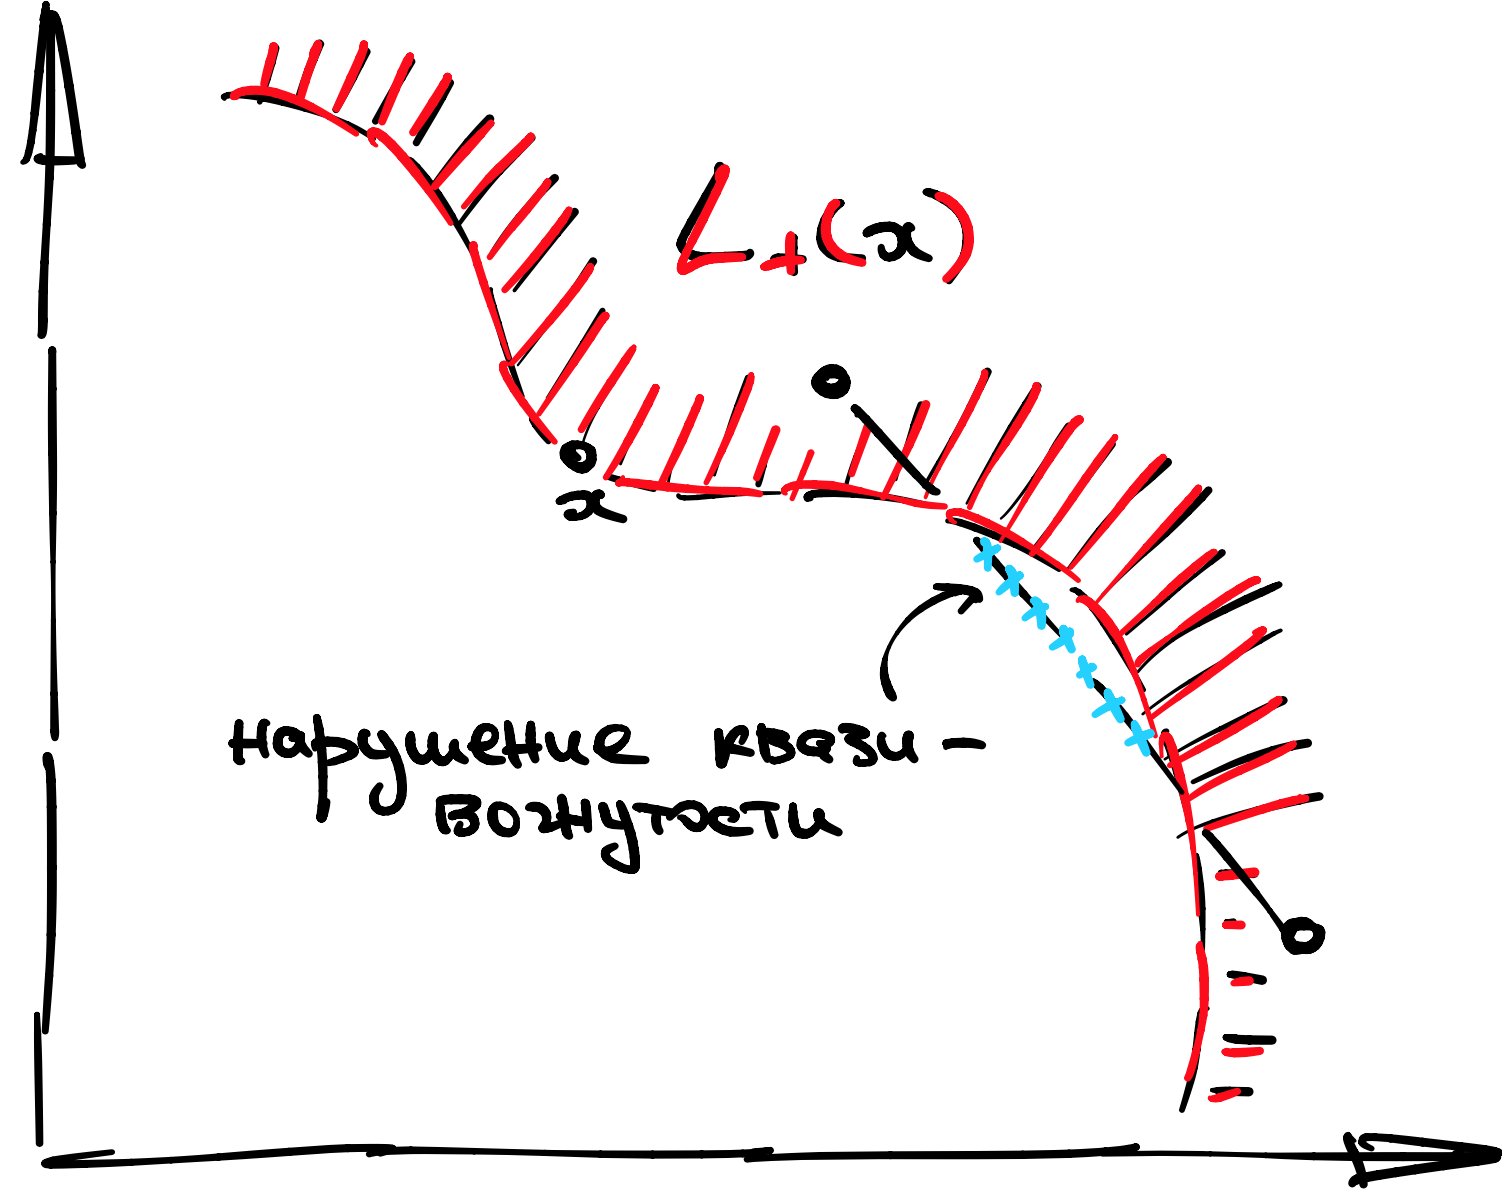
\includegraphics[width=.7 \textwidth]{not_quasi.png}
\end{figure}

\end{frame}

\begin{frame}{Вогнутость против квазивогнутости}

\begin{lemma}
Из вогнутости следует квазивогнутость, но не наоборот.
\end{lemma}

\begin{proof}
\begin{align*} 
(1) : & \quad U(\alpha x + (1-\alpha) y)) \geqslant \alpha U(x) + (1-\alpha) U(y) \\
(2) : & \quad \alpha U(x) + (1-\alpha) U(y) \geqslant \min (U(x), U(y))\\
(1), (2) \quad \Rightarrow & \quad U(\alpha x + (1-\alpha) y)) \geqslant \min (U(x), U(y))
\end{align*}
\end{proof}

P.S. Иногда я буду делать приставку <<\alert{строго}>>, это значит, что либо соответствующее множество строго выпукло, либо соответствующее неравенство строгое, смотрите на контекст.

\end{frame}

\section{Критика классической модели}

\begin{frame}{Неоднозначность полезности}

Для любого строго монотонного преобразования $\varphi$, две полезности - $U(x)$ и $\varphi(U(x))$ - производят идентичное поведение у потребителей.  

Довольно легко генерировать примеры идентичных функций, используя такие монотонные преобразования, как $\varphi(z) = z + c, cz , \log z$.
\begin{align*}
& x^2y^3,\\
& 2\log x + 3\log y,\\
& 2\log x + 3\log y + 1,\\
& 2(2\log x + 3\log y) + 1.
\end{align*}
Все выше перечисленные полезности эквивалентны.
\end{frame}

\begin{frame}{Неоднозначность вогнутости}

Вогнутость легко ломается при монотонных преобразованиях

\begin{lemma}
Если $U(x)$ вогнута, то $\varphi(U(x))$ квазивогнута для любого строго монотонного преобразования $\varphi$. 
\end{lemma}

Чтобы придумать доказательство, достаточно знать следующие свойства монотонных преобразований:
 \begin{align*}
U(x) \leqslant U(y) \quad \Leftrightarrow \quad \varphi(U(x)) \leqslant \varphi(U(y))\\
U(x) \geqslant U(y) \quad \Leftrightarrow \quad \varphi(U(x)) \geqslant \varphi(U(y))\\
\min(\varphi(U(x)), \varphi(U(y))) = \varphi(\min(U(x),U(y)))
\end{align*}

Попробуйте теперь написать доказательство самостоятельно.

\end{frame}

\begin{frame}{Неоднозначность вогнутости}

В отличие от вогнутости, квазивогнутость сохраняется при монотонных преобразованиях.

Это верно хотя бы потому, что определение вообще никак не опирается на форму графика полезности, а только на форму его Лебеговых множеств. А \alert{строго монотонные преобразования оставляют Лебеговы множества на месте}.

\begin{lemma}
Если $U(x)$ квазивогнута, то $\varphi(U(x))$ тоже квазивогнута для любого строго монотонного преобразования $\varphi$. 
\end{lemma}

Это делает ее гораздо более удобной, чем просто вогнутость.

\end{frame}

\section{Предпочтения}

\begin{frame}{Предпочтения}

Модель предпочтений еще более абстрактна

\begin{itemize}
\item снова один агент
\item товары разделены на $n$ категорий
\item портфель (потр. корзина) это точка в $\mathbb{R}_{+}^{n}$	
\item категории, а также координаты обозначаются $x, y, z...$
\item множество доступных альтернатив $X \subset \mathbb{R}_{+}^{n}$
\end{itemize}

Однако вместо полезности $U: X \to \mathbb{R}$ у агента в голове зашито бинарное предпочтение $\succcurlyeq: X^2 \to \{0,1\}.$ Что это значит?

\end{frame}

\begin{frame}{Предпочтения}

Проще всего визуализировать бинарное отношение на множестве альтернатив малой размерности, например 3.
$$
\begin{array}{c|ccc}
 \succcurlyeq & x & y & z\\
\hline
x & 1 & 1 & 0 \\
y & 0 & 1 & 1\\
z & 0 & 1 & 0
\end{array}
$$

$x \succcurlyeq y$ означает что $(x,y) \mapsto 1$.

$x \preccurlyeq y$ означает что $(y,x) \mapsto 1$.

Формально, бинарное отношение – это любое расположение ноликов и единичек внутри матрицы.

\end{frame}

\begin{frame}{Предпочтения}

Для простоты вводятся дополнительные обозначения:

$x \sim y$ означает что $x \succcurlyeq y$ и $x \preccurlyeq y$.

$x \succ y$ означает что $x \succcurlyeq y$ но не $x \sim y$.

$x \prec y$ означает что $x \preccurlyeq y$ но не $x \sim y$.

Получаются пять интуитивных отношений сильного, слабого предпочтений и безразличия.

Однако какие попало матрицы писать не стоит.

\end{frame}

\begin{frame}{Предпочтения}

Поскольку у бинарного отношения есть экономическая интерпретация, это накладывает на него определенные ограничения, называемые \alert{аксиомами рациональности}.

\begin{definition}
Предпочтения $\succcurlyeq$	\alert{рациональны}, если
\begin{itemize}
\item для любыx $x, y \in X$, хотя бы $x \succcurlyeq y$ либо $y \succcurlyeq x$.
\item для любой $x \in X$, всегда верно что $x \sim x$
\item для любыx $x, y, z \in X$: 
$$x \succcurlyeq y, y \succcurlyeq z \quad \Rightarrow \quad x \succcurlyeq z$$
\end{itemize}
\end{definition}
Последнее свойство - самое важное и называется \alert{транзитивностью}. 

\end{frame}

\begin{frame}{Предпочтения}

Рациональность накладывают структуру на то, как может заполняться матрица. 
$$ 
\begin{array}{c|ccc}
 \succcurlyeq & x & y & z\\
\hline
x & * & * & * \\
y & 0 & * & 1\\
z & 0 & 1 & *\\
\end{array}
$$
Попробуйте дозаполнить следующую матрицу так, чтобы предпочтения были рациональными.

\end{frame}

\section{Свойства предпочтений}

\begin{frame}{Предпочтения}

Переопределив Лебеговы множества $L_{+}(x)$ и $L_{-}(x)$ в терминах предпочтений, мы получаем непрерывность предпочтений.

\begin{definition}
Предпочтения $\succcurlyeq$ \alert{непрерывны} в $X$, если для любого $x \in X$ множества $L_{+}(x)$ и $L_{-}(x)$ замкнуты, где
$$L_{+}(x) = \{y \in X: y \succcurlyeq x\}, \quad L_{-}(x) = \{y \in X: y \preccurlyeq x\}$$
\end{definition}

И совершенно аналогично мы переносим квазивогнутость в мир предпочтений...

\end{frame}

\begin{frame}{Предпочтения}

... однако, вопреки логике, аналог термина квазиВОГНутости полезности в мире предпочтений называется ВЫПУклостью.

\begin{definition}
Предпочтения $\succcurlyeq$ \alert{выпуклы} в $X$, если $\forall x \in X$ множество $L_{+}(x)$ выпукло, то есть, оно содержит все свои хорды. 
\end{definition}

Парадокс в том, что вогнутые полезности - квазивогнутые, однако, ассоциированы с выпуклыми предпочтениями. 

А выпуклые полезности (которые еще надо отыскать) с выпуклыми предпочтениями вообще никак не связаны и даже скорее противоположны им. 

\end{frame}

\section{Прямая связь}

\begin{frame}{Прямая связь}

Предположим, что у вас уже есть откалиброванная полезность. Как вывести из нее модель предпочтений?

\begin{definition}
Будем говорить, что $U$ \alert{представляет} $\succcurlyeq$, если
$$ U(x) \geqslant U(y) \quad \Leftrightarrow \quad  x \succcurlyeq y.$$
\end{definition}

Это определение должно быть понятно на интуитивном уровне. 

Также должно быть понятно, что если предпочтения представлены $U$, то они будут обязательно рациональны, поскольку это просто свойства вещественных чисел.

\end{frame}

\section{Обратная связь}

\begin{frame}{Обратная связь}

Предположим, что у вас уже есть откалиброванные рациональные предпочтения. Можно ли восстановить по ним хотя бы одну непротиворечивую полезность? 

Оказывается, что в простых случаях, действительно, можно.

\begin{lemma}
Если $X$ конечно, то для любых рациональных предпочтений $\succcurlyeq$ существует полезность $U$, представляющая $\succcurlyeq$.
\end{lemma}

Это легко доказать алгоритмически.

В случае когда пространство альтернатив достаточно мощное, нам понадобится непрерывность предпочтений, и еще кое что.

\end{frame}

\begin{frame}{Обратная связь}

\begin{columns}
\begin{column}{0.5\textwidth}
   \alert{Жерар Дебрё} (Gérard Debreu) французский экономист и математик, профессор экономики университета Беркли, лауреат нобелевской премии 1983 года по экономике. Работал над \alert{представлениями предпочтений потребителя при помощи вещественнозначных функций} и существованием равновесий в конкурентных рынках.
\end{column}
\begin{column}{0.5\textwidth}  %%<--- here
    \begin{center}
     \includegraphics[width=1\textwidth]{debreu.jpg}
     \end{center}
\end{column}
\end{columns}

\end{frame}

\begin{frame}{Обратная связь}

\begin{theorem}[Дебрё]
Если $X\subset \mathbb{R}^n$ <<хорошее>>, то для любых рациональных и непрерывных предпочтений $\succcurlyeq$ существует непрерывная полезность $U$, представляющая $\succcurlyeq$.
\end{theorem}

<<Хорошесть>> - скучные технические условия связности и сепарабельности, так математики любят оформлять свои теоремы. По-настоящему важной здесь является именно непрерывность предпочтений.

Однако не стоит забывать, что, если предпосылки теоремы не выполнены, это еще не значит, что полезности нет. К примеру, дискретные пространства вовсе не связны.

\end{frame}

\section{Выбор}

\begin{frame}{Выбор}

Модель выбора максимально абстрактна

\begin{itemize}
\item снова один агент
\item товары разделены на $n$ категорий
\item портфель (потр. корзина) это точка в $\mathbb{R}_{+}^{n}$	
\item категории, а также координаты обозначаются $x, y, z...$
\item множество доступных альтернатив $X \subset \mathbb{R}_{+}^{n}$
\end{itemize}

Вместо полезности $U: X \to \mathbb{R}$...

или бинарного предпочтения $\succcurlyeq: X^2 \to \{0,1\}$...

у агента в голове зашито \alert{отображение выбора} $C: 2^X \to 2^X$. 

Что это значит?

\end{frame}

\begin{frame}{Выбор}

Это значит, что агент отображает подмножества в подмножества. Так же как и с предпочтениями, есть несколько естественных технических ограничений:

\begin{itemize}
  \item $C(Z) \neq \emptyset$
  \item $C(Z) \subset Z$
\end{itemize}

Для любого непустого меню $Z \subset X$. 

Есть еще третья, самая важная аксиома.

\end{frame}

\begin{frame}{Выбор}

Рассмотрим любые два портфеля $x, y \in X$ и два меню $Z,Z' \subset X$, таких что $x,y$ содержатся в обоих меню.

\begin{definition} 
\alert{Слабой аксиомой выбора} (WARP) называется следующее. 

Если в первом меню $Z$: $x_2$ был выбран в присутствии $x_1$, то втором меню $Z'$ невозможно чтобы: $x_1$ был выбран в присутствии $x_2$, но сам $x_2$ при этом выбран не был.
\end{definition}

Читая это определение задом наперед, можно интуитивно понять, что оставляя $x_1$ но исключая $x_2$ внутри меню $Z'$ вы, по сути, озвучиваете строгое предпочтение $x_1 \succ x_2$. И в других меню вам запрещается вести себя в противоречии с этим предпочтением.

\end{frame}

\begin{frame}{Выбор}

Если будет время, я выведу слабую аксиому выбора из рациональности предпочтений, когда агент строит свой выбор оптимизируя предпочтения по конечному числу элементов. 

Это будет аналог прямой связи между предпочтениями и выбором.
%
%Для обратной связи понадобится так называемая \alert{обобщенная аксиома выбора} (GARP), которая говорит что если $x_2$ был выбран в присутствии $x_1$, а $x_3$ был выбран в присутствии $x_2$ и так по цепочке...  $x_n$ был выбран в присутствии $x_{n-1}$, то невозможно, чтобы $x_1$ был выбран в присутствие $x_n$, но сам $x_n$ при этом выбран не был.
%
%Это звучит немножко как транзитивность предпочтений, но гораздо глубже, это очень продвинутый материал.

\end{frame}

\section{Перед тем как уйти на перерыв}

\begin{frame}{Заключение}

Мы продемонстрировали, что из любой полезности можно вывести рациональные предпочтения, а из рациональных предпочтений выбор со слабой аксиомой.

С другой стороны, из любых непрерывных и рациональных предпочтений можно вывести непрерывную полезность - это Теорема Дебре.

Аналог обратной связи для выбора я рассказывать не буду, это называется \alert{Теорема Африата}, это очень продвинутый материал, и там понадобится усиленная аксиома выбора (GARP) которая не входит в мой курс. 

\end{frame}

\begin{frame}{Заключение}

\begin{figure}[hbt]
\centering
\includegraphics[width=1 \textwidth]{arch.png}
\end{figure}

\end{frame}

\begin{frame}{Заключение}

Какой из всего этого можно сделать вывод?

Все три модели, в каком то смысле эквивалентны. Поэтому можно смело использовать ту, которая вам кажется удобнее. 

Чаще всего (99\% случаев) это полезность, но иногда это и предпочтения, например в анализе алгоритма Гейла-Шепли, при помощи которого вас распределили по факультетам. 

С другой стороны, аксиомы выбора недавно <<вылезли>> в новейших комбинаторных аукционах, поэтому от теории выбора тоже есть некоторый толк.

\end{frame}

\section{Конец первой части лекции}

\begin{frame}{План на вторую часть лекции (1 час)}

Далее мы сфокусируемся только на полезностях и как оптимизировать их при различных ограничениях.

\begin{itemize}
  \item Начала оптимизации
  \item Условия первого и второго порядка
  \item Выпуклость задачи
  \item Краевые и внутренние решения
  \item Линии уровня и геом. анализ
\end{itemize}


\end{frame}

\section{Начала оптимизации}

\begin{frame}{Начала оптимизации}

Любая оптимизационная задача – это две вещи:

\begin{itemize}
  \item функция $U$ которую мы максимизируем
  \item область определения $X$ по которым мы максимизируем
\end{itemize}

Ключевыми факторами тут являются непрерывность и (квази-) вогнутость целевой функции, а также компактность и выпуклость области определения.

\end{frame}

\section{Существование}

\begin{frame}{Существование}

Существование решения, как правило, мы можем легко гарантировать при помощи следующей теоремы

\begin{theorem}[Вейерштрасса]

Непрерывная функция на (непустом) компакте гарантированно достигает своего минимума и максимума.
\end{theorem}

Что такое \alert{непрерывность} вы уже знаете, а \alert{компакт} в $\mathbb{R}^n$ - это просто ограниченное и замкнутое множество. 

В контексте одномерной оптимизации, отрезок $[a,b]$ - это компакт, а $(a,b]$, $[a,b)$, $(a,b)$, $[a,\infty)$,$(a,\infty)$ - нет. 

В экономике вам будут попадаться, в основном компакты, поэтому вопрос о существовании как правило стоит не остро.

\end{frame}

\section{Дифференциальный анализ}

\begin{frame}{Дифференциальный анализ}

Предположим, что функция на компакте не только непрерывна но еще и дифференциируема сколько угодно раз, такая задача называется \alert{гладкой}. Тогда оптимум может быть

\begin{itemize}
  \item либо на границе $X$
  \item либо во внутренней точке $X$
\end{itemize}

В последнем случае обязательно выполнены \alert{условия первого порядка} (УПП), это один из самых фундаментальных результатов дифференциального анализа.

\end{frame}

\begin{frame}{УПП}

Например, если функция $U(x, y, z)$ от трех переменных, и вы убедили себя, что решение надо искать внутри, то
$$\text{УПП (FOC)}: \quad  \nabla U = 0$$ 
должны выполняться в оптимальной точке $(x^{\ast}, y^{\ast}, z^{\ast})$. 

Значок $\nabla$ означает взятие градиента функции $$ \nabla U = \begin{pmatrix} \partial U/\partial x \\ \partial U/\partial y \\ \partial U/\partial z \end{pmatrix}$$
в соответствующей точке.

\end{frame}

\begin{frame}{УПП на границе}

Например, если функция $U(x, y, z)$, и вы убедили себя, что решение надо искать на границе $F(x,y,z) = 0$, то
$$\text{УПП (FOC)}: \quad  \nabla \mathcal{L} = 0, $$ 
где $\mathcal{L}(x,y,z|\lambda) = U(x, y, z) - \lambda F(x,y,z)$ это \alert{Лагранжиан}.

Значок $\nabla$ означает взятие градиента Лагранжиана по всем переменным включая множители Лагранжа $$ \nabla \mathcal{L} = \begin{pmatrix} \partial \mathcal{L}/\partial x \\ \partial \mathcal{L}/\partial y \\ \partial \mathcal{L}/\partial z \\ \partial \mathcal{L}/\partial \lambda \end{pmatrix}$$
в соответствующей точке.

\end{frame}


\begin{frame}{Критические точки}

Как правило, количество точек, в которых выполнены УПП, с Лагранжианом или без,  конечно. Оптимум может также находиться на каком-то изломе или иной аномалии границы области определения.

Все такие точки называются \alert{критическими}, их мало, и оптимум гарантированно лежит в одном из них. 

\end{frame}

\begin{frame}{Критические точки}

\begin{figure}[hbt]
\centering
\includegraphics[width=.8 \textwidth]{extrema.png}
\end{figure}

\end{frame}

\begin{frame}{Ручной перебор}

Если у вас по любой причине остался один кандидат, то он и является оптимумом, поскольку существование нам гарантирует Теорема Вейерштрасса. 

Если же кандидатов несколько, то надо сравнивать значения функции руками и выбирать все точки с наибольшим значением. 

Тупой перебор Критические точки может привести к неожиданно быстрому решению задачи.

\end{frame}

\begin{frame}{Пример 1}

Промаксимизируем функцию $f(x) = (x-1)^2$ на отрезке $[0,3]$.

\begin{itemize}
  \item Задача гладкая на компакте
  \item Решим УПП, получим первую критическую точку $x = 1$
  \item Две других критические точки это $x = 0$ и $x = 3$
  \item Сравним значения: $$f(0) = 1, \ f(1) = 0, \ f(3) = 4.$$
\end{itemize}

Получается, что в этой задаче один единственный оптимум в точке $x = 3$, причем до условий второго порядка у нас даже руки не дошли.

\end{frame}

\begin{frame}{УВП}

Число внутренних точек, прошедших УПП, можно дополнительно сузить за счет условий второго порядка.
$$\text{УВП (SOC)}: \quad  \nabla^2 U \ ? \ 0$$
Если Гессиан во внутренней точке отрицательно полу-определен $\nabla^2 U \leqslant 0$ (собственные значения $\leqslant 0$), то это \alert{локальный максимум} и этот кандидат проходит отбор.

Если Гессиан положительно определен $\nabla^2 U > 0$ (собственные значения $>0$), то это строгий \alert{локальный минимум} и этот кандидат точно не проходит отбор.

Есть еще третий случай, когда собственные значения Гессиана имеют противоположные знаки, это \alert{седло} и оно тоже не проходит отбор.

\end{frame}

\section{Выпуклость}

\begin{frame}{Выпуклость}

К счастью, в экономике зачастую удается показать, что поверх непрерывности функция полезности

\begin{itemize}
\item либо вогнутая
\item либо она монотонное преобразование вогнутой
\item либо она квазивогнутая
\end{itemize}

Если, вдобавок, область определения - выпуклое множество, то условия второго порядка можно не проверять. Такие задачи называются \alert{выпуклыми}.

\end{frame}

\begin{frame}{Пример 2}

Промаксимизируем функцию $f(x) = -(x-1)^2$ на отрезке $[0,3]$.

\begin{itemize}
  \item Задача гладкая и выпуклая на компакте
  \item Решим УПП, получим первую критическую точку $x = 1$
  \item Убедимся что он находится внутри области
\end{itemize}

Все, этот экстремум и есть решение.

\end{frame}

\begin{frame}{Пример 3}

Промаксимизируем функцию $f(x) = -(x+1)^2$ на отрезке $[0,3]$.

\begin{itemize}
  \item Задача гладкая и выпуклая на компакте
  \item Решим УПП, получим первую критическую точку $x = -1$
  \item Однако он не попадает в область, то есть, его нет
  \item Две других критических точки это $x = 0$ и $x = 3$
  \item Сравним значения: $$f(0) = 1, \ f(3) = -16.$$
\end{itemize}

Получается, что в этой задаче один единственный оптимум в точке $x = 0$.

\end{frame}

\begin{frame}{Выпуклость}

Очень важно уметь, глядя на задачу, определять выпуклая она или нет, чтобы не тратить время на анализ второго порядка. 

Общий алгоритм решения гладких и выпуклых задач на компакте очень простой:

\begin{itemize}
\item ищем первую критическую точку, как будто решение внутреннее
\item если не попало в область определения - ищем на границе
\item не забываем про изломы и иные аномалии области определения, потому что они, формально, являются кандидатами на решение
\end{itemize}

\alert{В выпуклых задачах условия второго порядка выполнены автоматически}, их проверка - пустая трата времени.

\end{frame}

\section{Геометрический анализ}

\begin{frame}{Линии уровня}

Наконец, линии уровня - это очень удобный инструмент для быстрого отлова и классификации кандидатов на решение оптимизационной задачи...

\begin{definition}
\alert{Линией уровня} полезности $U$, проходящей через точку $x$ называется множество всех точек $y \in X$ таких, что $U(y) = U(x)$.
\end{definition}

... особенно в двумерном случае.

\end{frame}

\begin{frame}{Кривые безразличия}

\begin{definition}
\alert{Кривой безразличия} предпочтений $\succcurlyeq$, проходящей через точку $x$ называется множество всех точек $y \in X$ таких, что $x \sim y$. Другими словами, это пересечение $L_+(x)$ и $L_-(x)$.
\end{definition}

Совершенно ясно, что в контексте представлений предпочтений полезностями, кривая безразличия и линия уровня - это одно и то же.

\end{frame}

\section{Локальная ненасыщаемость}

\begin{frame}{Локальная ненасыщаемость}

\begin{definition}
Предпочтения $\succcurlyeq$ \alert{локально ненасыщаемы} в $X$, если для любой точки $x \in X$ найдется сколь угодно близкая к ней точка $x' \in X$, такая что $x' \succ x$.
\end{definition}

\begin{definition}
Полезность $U$ \alert{локально ненасыщаема} в $X$, если для любой точки $x \in X$ найдется сколь угодно близкая к ней точка $x' \in X$, такая что $U(x') > U(x)$.
\end{definition}

Почти все полезности, которые будут вам встречаться, локально ненасыщаемы. Интуитивно это означает что кривые безразличия - тонкие линии. Если кривая безразличия толстая - это явное нарушение локальной ненасыщаемости.

\end{frame}

\section{Примеры полезностей}

\begin{frame}{Линейная полезность}

Рассмотрим полезность вида: $U(x, y) = ax + by$. Тогда линия уровня ищется следующим образом: 
\begin{gather*}
c = ax + by\\
c-ax = by\\
y = \frac{c-ax}{b}
\end{gather*}
Линия уровня - это прямая вида $y = \alpha x + \beta$.

Эта полезность гладкая, вогнутая и локально ненасыщаемая.

\end{frame}

\begin{frame}{Гиперболическая полезность}

Рассмотрим полезность вида: $U(x, y) = a \log x + \log y$. Тогда линия уровня ищется следующим образом: 
\begin{gather*}
c =  a \log x + \log y\\
e^{c} = x^a y\\
y =\frac{e^{c}}{x^a}
\end{gather*}
Линия уровня - это гипербола вида $y = x^\alpha \beta$.

Эта полезность гладкая, вогнутая и локально ненасыщаемая.

\end{frame}

\begin{frame}{Полезность минимум}

Рассмотрим полезность вида: $U(x, y) = \min(ax, by)$. Тогда линия уровня ищется следующим образом: 
\begin{gather*}
c = \min(ax, by)\\
\frac{c}{b}= \min(\frac{a}{b}x, y), \quad \frac{c}{a}= \min(x, \frac{b}{a}y)\\
y = \frac{c}{b} \mathbb{I}(ax > c), \quad x = \frac{c}{a} \mathbb{I}(by > c)
\end{gather*}
Линия уровня - это конкатенация горизонтальной и вертикальной линий, соединенных вдоль $ax = by$.

Эта полезность НЕгладкая, но непрерывная, вогнутая и локально ненасыщаемая.

\end{frame}

\section{Метод пристального взгляда}

\begin{frame}{Метод пристального взгляда}

Очень часто, в задачах есть выпуклое ограничение типа неравенства, например, бюджетное ограничение. A полезность вогнутая или квазивогнутая.

В таком случае, оптимум можно охарактеризовать как точку касания выпуклой области определения с одним из выпуклых верхних Лебеговых множеств. Однако, \alert{метод пристального взгляда работает только для локально ненасыщаемых предпочтений}. 

В маломерных задачах, эта точка ищется визуально, а точные ее координаты либо угадываются из симметрии, либо из каких то других соображений.

\end{frame}

\begin{frame}{Метод пристального взгляда}

\begin{figure}[hbt]
\centering
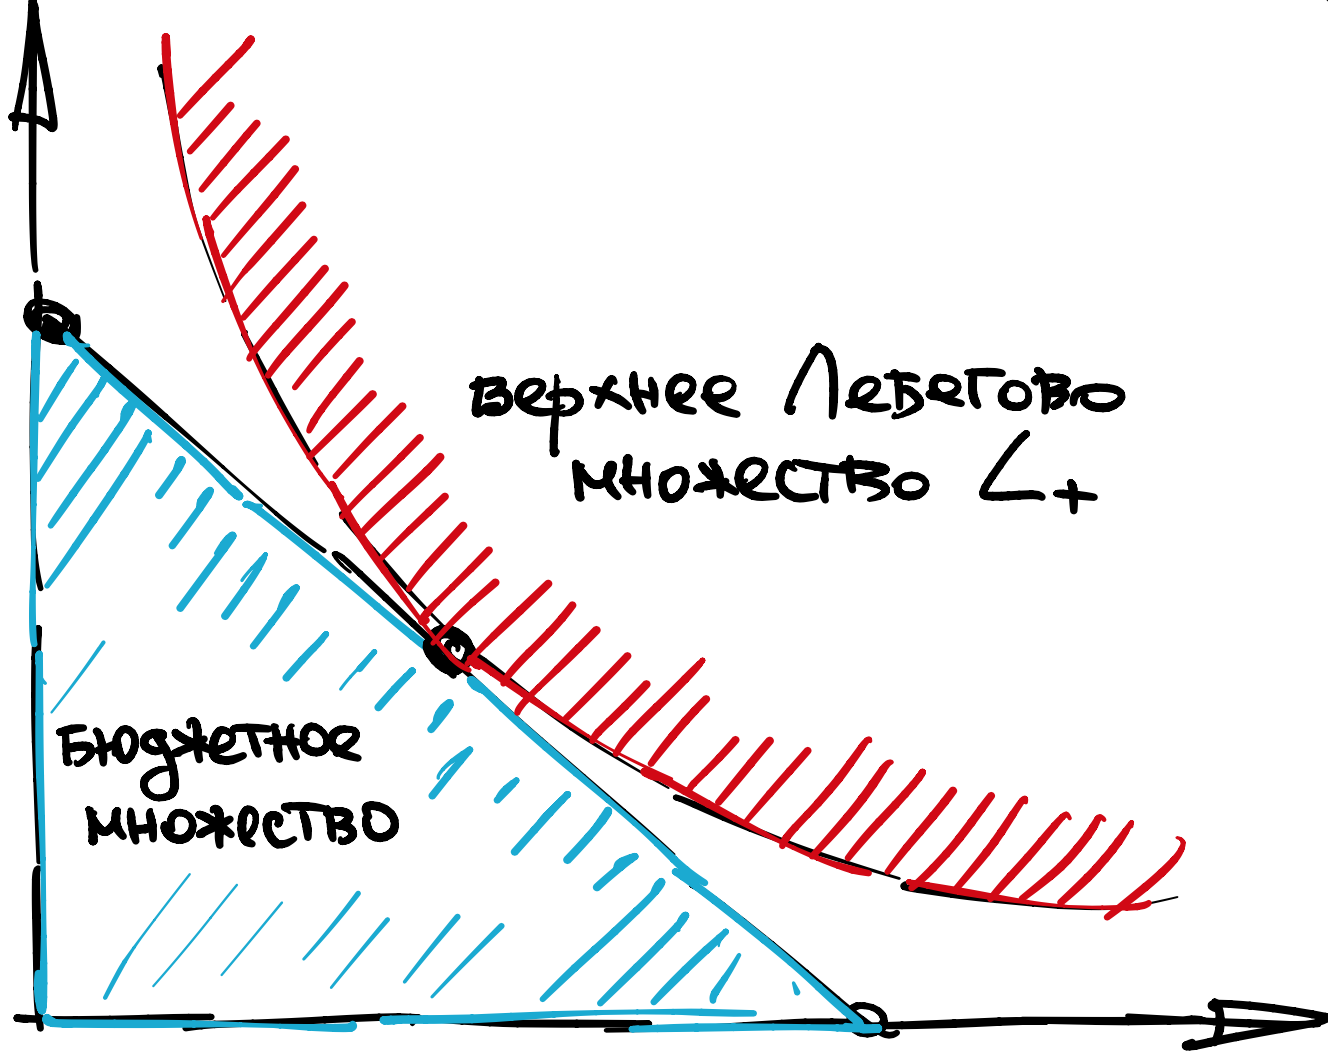
\includegraphics[width=.8 \textwidth]{tangency.png}
\end{figure}

\end{frame}
\begin{frame}{Метод пристального взгляда}

\begin{figure}[hbt]
\centering
\includegraphics[width=.8 \textwidth]{tang2.png}
\end{figure}

\end{frame}
\begin{frame}{Метод пристального взгляда}

\begin{figure}[hbt]
\centering
\includegraphics[width=.8 \textwidth]{tang3.png}
\end{figure}

\end{frame}

\section{Конец второй части лекции}

\end{document}